%# -*- coding: utf-8 -*-
\input{ctex4xetex.cfg}
\documentclass[cs4size,oneside,openany]{ctexbook}
\linespread{1.0}

%\includeonly{xiantu}

\usepackage{amsmath}

\usepackage{makeidx}
\makeindex

\usepackage{geometry}
\geometry{screen,left=0.5cm,right=0.5cm,top=2cm,bottom=1cm}

\usepackage{fancyhdr}
\renewcommand{\headrulewidth}{0pt}
\pagestyle{fancy}
\fancyhf{}
\lhead{\normalfont\rightmark}
\rhead{\normalfont\thepage}
\fancypagestyle{plain}{\fancyhf{}}

\usepackage{float}
\floatplacement{htbp}
\AtBeginDocument{
  \renewcommand{\topfraction}{0.9} % default 0.7
  \renewcommand{\bottomfraction}{0.5} % default 0.3
  \renewcommand{\textfraction}{0.1} % default 0.2
  \renewcommand{\floatpagefraction}{0.8} % default 0.5
  \setlength{\floatsep}{3pt plus 1pt minus 1pt} % default 12pt plus2pt minus2pt
  \setlength{\textfloatsep}{6pt plus 1pt minus 1pt} % default 20pt plus2pt minus4pt
  \setlength{\intextsep}{3pt plus 1pt minus 1pt} % default 12pt plus2pt minus2pt
}

\usepackage{caption}
\captionsetup{skip=6pt} % default 10pt

\usepackage{xltxtra}
\usepackage{myfonts}

\usepackage{multicol}

\usepackage{xcolor}
\pagecolor{lightgray!50}

\usepackage{asymptote}
\usepackage{graphicx}
\usepackage{hyperref}
\hypersetup{
  bookmarksopen=false,
  pdfpagemode=FullScreen,
  colorlinks=false,
  pdfborder=0 0 0
}
\renewcommand\figureautorefname{图}

\usepackage{asysyntex}
\usepackage{listings}
\lstloadlanguages{[LaTeX]TeX}
\newcommand*\texcode{\expandafter\lstinline[language={[LaTeX]TeX}]}


\newcommand*\prgname[1]{\textsf{#1}}
\newcommand*\Asy{\textsf{Asymptote}}
\newcommand*\asyversion{1.70}
\begin{document}

\frontmatter

% 标题页
\begin{titlepage}
\vspace*{\stretch{1}}
\begin{center}
  {\zihao{2}\bfseries
  \Asy\ 范例教程}
\bigskip

  {\zihao{3}\sffamily
  milksea}
\bigskip

  {\today}
\end{center}
\vspace*{\stretch{3}}
\end{titlepage}

% 版权页
\begingroup
\setlength{\parindent}{0pt}
\vspace*{\stretch{1}}
本文是基于 \Asy\ \asyversion{} 的一组教程。

\url{http://asy4cn.googlecode.com/}
\medskip

版权所有\copyright\ 2009 milksea, milksea@163.com

{\setlength{\leftskip}{2em}
在 GNU General Public License(GNU 通用公共许可证)的条款下授予复制、发布和/或修改此文档的许可。许可证条款见附录 \ref{chap:license}。\par}
\endgroup
\newpage

\mainmatter

%# -*- coding: utf-8 -*-
% xiantu.tex
% asymptotebyexample 的一章,最基础的画图知识

\chapter{赵爽的弦图}
\label{chap:xiantu}

赵爽博士是位老知识分子,研究兴趣是天文历法与算学,一生精研《周髀算经》。不过
赵老爷子年轻的时候书籍都是手写,最近才紧跟时代潮流用上了电脑。现在他要修订他
研究《周髀算经》的札记,决定使用 \LaTeX{} 来排版。

现在他遇到一个难题,就是他要画出笔记中讲解勾股定理的一幅弦图。听人介绍,几经
比较之后,他决定使用现在炒得火热的 \Asy{}。

赵博士的原图是手画的,线框多有不直不准的,\autoref{fig:xiantuancient} 就是旧
年据手稿做的雕版图,赵博士并不满意。赵爽博士理想中的图,线条要平整美观,文字
要清楚整齐,图形还要上色:朱实自然得用红色,黄实也该用黄色,以与注文一致——
就是\autoref{fig:xiantu} 的样子。

\begin{figure}
  \centering
  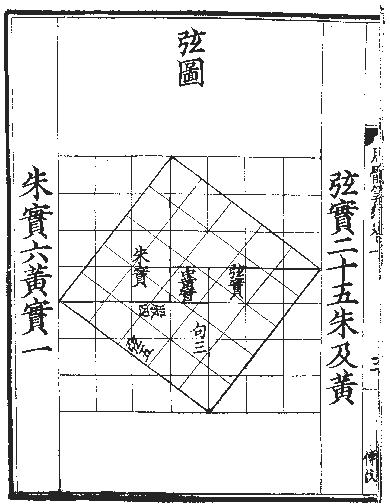
\includegraphics[height=\textheight-2\baselineskip]{xiantu-ancient.pdf}
  \caption{旧年做的雕版}
  \label{fig:xiantuancient}
\end{figure}
\begin{figure}
  \centering
  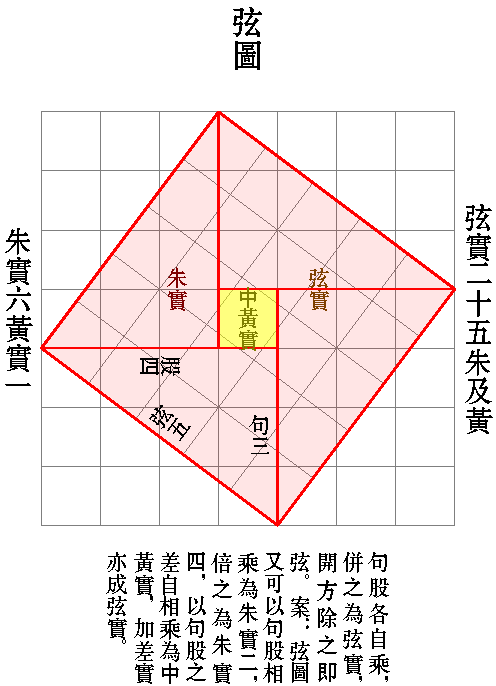
\includegraphics{xiantu.pdf}
  \caption{理想中的新版本}
  \label{fig:xiantu}
\end{figure}

计议已定,赵博士要开始正式的绘图了。

\section{绘图环境}

\Asy{} 的安装并不复杂,在 Windows 下面就是下载运行那个安装包,在 Linux 下面一
般也只需要下载对应的压缩包,解压就可以使用了。哦,赵博士用的就是 Windows。

点图标运行 \Asy{},就出现了交互式\index{交互式}的命令行,提示符是一个
\verb=>=。输入命令:
\begin{lstlisting}
draw((0,0) -- (3cm,4cm));   // `\color{comment}一条直线`
\end{lstlisting}
赵博士装的 GSView 立即弹了出来,里面已经画出一条倾斜的直线。再输入
|quit|\index{quit@\lstinline=quit=},程序退出,并留下了一个叫做
\verb=out.eps= 的图形文件,
小菜一碟。

这里稍稍解释一下上面的一句代码。|draw|\index{draw@\lstinline=draw=} 是画线的
命令,更准确地说,是 \Asy{} 中的函数\index{函数}:它带有一个参数\index{参数}
|(0,0) -- (3cm,4cm)|,参数外面是圆括号,整个命令以分号结束。里面的
|(0,0) -- (3cm,4cm)| 是由两个坐标\index{坐标}连接而成的直线,坐标是在直角坐标
系下的,可以带单位 |mm|, |cm|, |pt|, |bp|, |inch|, |inches|,%
\index{mm@\lstinline=mm=}\index{cm@\lstinline=cm=}\index{pt@\lstinline=pt=}%
\index{bp@\lstinline=bp=}\index{inch@\lstinline=inch=}%
\index{inches@\lstinline=inches=}%
其意义与在\TeX{} 中的一样,如果不带单位,则默认为 |bp|。行末以 |//| 开头的是
注释,另有一种在 |/* */| 之间的注释\index{注释},与 C 语言相同。

\index{编译}
不过赵博士写书讲求胸有成竹方才下笔,因此他更愿意使用更一种方式:打开一个文本
编辑器,把上面的绘图命令都录入完毕,保存为一个名为 \verb=line.asy= 的文件,最
后把这个文件拖动到 \Asy{} 的图标上面,就完成了整个作图。

赵博士的小侄子不屑于这种快捷图标的编译方式,他直接进入命令行,输入
\verb=asy=,就进入了 \Asy{} 的交互环境;要是输入 \verb=asy line=,就画出了刚
才的保存的直线。


\section{直线与绘图命令}
\label{sec:linedraw}

弦图的图形其实很简单,都是直线、方块、三角形这些,而且为了计算的简便,所有长
度也都是整数值。那么,首先就是在 \Asy{} 中来画直线。

\index{画线}
正如前面试验的时候做的那样,一条直线就是用 |--|\index{--@\lstinline=--=} 把坐
标连起来,再使用 |draw| 命令,直线就画出来了。事实上,可以用 |--| 把坐标点连
成折线:
\begin{lstlisting}
draw( (0,0) -- (1cm,0) -- (2cm,0.5cm) -- (1cm,1cm) -- (0,1cm) );
\end{lstlisting}
\begin{figure}[H]
\centering
\begin{asy}
draw( (0,0) -- (1cm,0) -- (2cm,0.5cm) -- (1cm,1cm) -- (0,1cm) );
\end{asy}
\end{figure}

像这样把坐标用 |--| 连结起来的,就成为一条路径\index{路径}。把直线而稍做修改
,在后面连上一个特殊的坐标 |cycle|\index{cycle@\lstinline=cycle=},就可以得到
一条首尾相接的闭路径\index{路径!闭路径}。如:
\begin{lstlisting}
draw( (0,0) -- (1cm,0) -- (2cm,0.5cm) -- (1cm,1cm) -- (0,1cm) -- cycle );
\end{lstlisting}
\begin{figure}[H]
\centering
\begin{asy}
draw( (0,0) -- (1cm,0) -- (2cm,0.5cm) -- (1cm,1cm) -- (0,1cm) -- cycle );
\end{asy}
\end{figure}

画一条路径可以使用不同的颜色、粗细的笔,这只要给 |draw| 命令多加一个画笔
\index{画笔}参数(多个参数用逗号分开):
\begin{lstlisting}
draw((0,0) -- (1cm,0) -- (2cm,0.5cm) -- (1cm,1cm) -- (0,1cm), darkblue+1mm);
\end{lstlisting}
\begin{figure}[H]
\centering
\begin{asy}
draw((0,0) -- (1cm,0) -- (2cm,0.5cm) -- (1cm,1cm) -- (0,1cm), darkblue+1mm);
\end{asy}
\end{figure}
这里 |darkblue| 是颜色,|1mm| 是线的粗细。|darkblue+1mm| 即指一毫米宽的深
蓝色粗线。(可用的颜色\index{颜色}名称可以参考 \cite{asyman})

赵博士画的是“勾三股四弦五”的红色三角形,这很容易:
\begin{lstlisting}
draw( (0,0) -- (4cm,0) -- (0,3cm) -- cycle, red+0.5mm );
\end{lstlisting}
\begin{figure}[H]
\centering
\begin{asy}
draw( (0,0) -- (4cm,0) -- (0,3cm) -- cycle, red+0.5mm );
\end{asy}
\end{figure}

\index{填充}
不过现在还需要的是实心的三角形,因此就需要一个新的绘图命令
|fill|\index{fill@\lstinline=fill=},即填充。于是,红色三角形就成为
\begin{lstlisting}
fill( (0,0) -- (4cm,0) -- (0,3cm) -- cycle, red );
\end{lstlisting}
\begin{figure}[H]
\centering
\begin{asy}
fill( (0,0) -- (4cm,0) -- (0,3cm) -- cycle, red );
\end{asy}
\end{figure}

但这样一来三角形的颜色就太重了,而且边界也不清楚。因此似乎应该先用浅红色填充
一遍,然后再用深红色勾边。好在可以使用一个命令
|filldraw|\index{filldraw@\lstinline=filldraw=} 同时完成这两件事情,这样就不
需要把一条路径写两遍了。即有:
\begin{lstlisting}
filldraw((0,0) -- (4cm,0) -- (0,3cm) -- cycle,
    fillpen=palered, drawpen=red+0.5mm);
\end{lstlisting}
\begin{figure}[H]
\centering
\begin{asy}
filldraw((0,0) -- (4cm,0) -- (0,3cm) -- cycle,
    fillpen=palered, drawpen=red+0.5mm);
\end{asy}
\end{figure}
这里可以简单地直接写两个参数 |palered, red+0.5mm|,不过为了清晰起见还是使用
“$\text{键}=\text{值}$”的写法,明确表示出填充的画笔和描线的画笔。

现在,赵博士的整个弦图的框架就呼之欲出了,就是画出四个三角形
(\autoref{fig:xiantuskeleton}):
\begin{lstlisting}
filldraw( (4cm,0) -- (4cm,3cm) -- (0,3cm) -- cycle,
    fillpen=palered, drawpen=red+0.5mm);
filldraw( (7cm,4cm) -- (4cm,4cm) -- (4cm,0) -- cycle,
    fillpen=palered, drawpen=red+0.5mm);
filldraw( (3cm,7cm) -- (3cm,4cm) -- (7cm,4cm) -- cycle,
    fillpen=palered, drawpen=red+0.5mm);
filldraw( (0,3cm) -- (3cm,3cm) -- (3cm,7cm) -- cycle,
    fillpen=palered, drawpen=red+0.5mm);
\end{lstlisting}
\begin{figure}
\centering
\begin{asy}
filldraw( (4cm,0) -- (4cm,3cm) -- (0,3cm) -- cycle,
    fillpen=palered, drawpen=red+0.5mm);
filldraw( (7cm,4cm) -- (4cm,4cm) -- (4cm,0) -- cycle,
    fillpen=palered, drawpen=red+0.5mm);
filldraw( (3cm,7cm) -- (3cm,4cm) -- (7cm,4cm) -- cycle,
    fillpen=palered, drawpen=red+0.5mm);
filldraw( (0,3cm) -- (3cm,3cm) -- (3cm,7cm) -- cycle,
    fillpen=palered, drawpen=red+0.5mm);
\end{asy}
\caption{弦图的初步框架}\label{fig:xiantuskeleton}
\end{figure}

还应该画出弦图的中间的“黄实”,用黄色填充。这部分是一个正方形,可以使用现成
的 \lstinline[mathescape]|box($\text{角点}$, $\text{角点}$)|
\index{box@\lstinline=box=} 命令来产生矩形的路径,因而填充正中间的正方形就可
以用:
\begin{lstlisting}
fill( box((3cm,3cm), (4cm,4cm)), yellow );
\end{lstlisting}
这个填充的命令应该放在画线之前(以免覆盖描的红线)。

回顾前面的代码,赵博士觉得连续地写四个 |filldraw| 命令太重复了。他读了 \Asy{}
的文档 \cite{asyman},才知道多条路径可以用符号 |^^|\index{^^@\lstinline=^^=} 
连起来,一起使用,于是立即着手改进原来的代码。

而且,由于还打算在图的后面画出参考网格,图形的颜色还应该设置为半透明\index{透
明}的。好在这并不难实现,只要稍稍改动一下填充的画笔,使用
\lstinline[mathescape]|opacity($\text{数值}$)|
\index{opacity@\lstinline=opacity=}
来设定有一定不透明度(取值为 $0\sim1$)的画笔,并把它加在原来的画笔上
\footnote{\Asy{} 的 EPS 格式输出看不到透明效果,必须输出为 PDF 格式或从 PDF 
格式转化为其他格式才能有透明效果。}。于是赵博士最后写出了这样的代码:
\begin{lstlisting}
fill( box((3cm,3cm), (4cm,4cm)), opacity(0.5)+yellow );
filldraw( (4cm,0) -- (4cm,3cm) -- (0,3cm) -- cycle
    ^^ (7cm,4cm) -- (4cm,4cm) -- (4cm,0) -- cycle
    ^^ (3cm,7cm) -- (3cm,4cm) -- (7cm,4cm) -- cycle
    ^^ (0,3cm) -- (3cm,3cm) -- (3cm,7cm) -- cycle,
    fillpen=opacity(0.1)+red, drawpen=red+0.5mm );
\end{lstlisting}
至此,弦图的主要框架(\autoref{fig:xiantuskeleton2})就此完成。
\begin{figure}[H]
\centering
\begin{asy}
fill( box((3cm,3cm), (4cm,4cm)), opacity(0.5)+yellow );
filldraw( (4cm,0) -- (4cm,3cm) -- (0,3cm) -- cycle
    ^^ (7cm,4cm) -- (4cm,4cm) -- (4cm,0) -- cycle
    ^^ (3cm,7cm) -- (3cm,4cm) -- (7cm,4cm) -- cycle
    ^^ (0,3cm) -- (3cm,3cm) -- (3cm,7cm) -- cycle,
    fillpen=opacity(0.1)+red, drawpen=red+0.5mm );
\end{asy}
\caption{弦图的进一步优化的框架}\label{fig:xiantuskeleton2}
\end{figure}


\section{图形变换与功能模块的使用}
\label{sec:transformmodule}

然后是画作为长度参考的网格。其实网格一开始就该在图中画出来,这样后面画图准确
与否才能看得清楚。不过现在赵博士是重作旧图,图样已定,网格就搁在弦图的主要图
形后面才画了。

按说这个网格是十分简单的,无非就是画一些灰色的纵横细线。比如这个 $3\times3$ 
的网格:
\begin{lstlisting}
draw( (0,0) -- (3cm,0)
    ^^ (0,1cm) -- (3cm,1cm)
    ^^ (0,2cm) -- (3cm,2cm)
    ^^ (0,3cm) -- (3cm,3cm),
    gray );
draw( (0,0) -- (0,3cm)
    ^^ (1cm,0) -- (1cm,3cm)
    ^^ (2cm,0) -- (2cm,3cm)
    ^^ (3cm,0) -- (3cm,3cm),
    gray );
\end{lstlisting}
\begin{figure}[H]
\centering
\begin{asy}
draw( (0,0) -- (3cm,0)
    ^^ (0,1cm) -- (3cm,1cm)
    ^^ (0,2cm) -- (3cm,2cm)
    ^^ (0,3cm) -- (3cm,3cm),
    gray );
draw( (0,0) -- (0,3cm)
    ^^ (1cm,0) -- (1cm,3cm)
    ^^ (2cm,0) -- (2cm,3cm)
    ^^ (3cm,0) -- (3cm,3cm),
    gray );
\end{asy}
\end{figure}

可无疑这个办法显得太麻烦了,赵博士要画的是 $7\times7$ 的网格,就要分别画出
$16$ 条直线。这样的代码不仅不好写,而且容易出错,修改一下也很麻烦。

赵博士看到了手册 \cite{asyman} 中讲循环语句的用法,似乎可以完成这件事。可是以
赵博士的年龄,再去看什么编程什么变量的,命令不能一条一条执行下来,很不习惯,
头脑就往往转不清楚。

\index{模块!math@\prgname{math}}
于是赵博士就去论坛上咨询,一些人劝他去用几行循环语句,甚至有人已经把完整的函
数做好了。但有一个结果特别引人注目,有人指出,在 \prgname{math} 模块中已经定
义好了一个 |grid| 函数,只要拿来用就可以了。赵博士立即精神大振,来看这个
|grid| 函数:\index{grid@\lstinline=grid=}
\begin{lstlisting}
picture grid(int Nx, int Ny, pen p=currentpen)
\end{lstlisting}
这个是在 \prgname{math} 模块中 |grid| 函数的原型。\index{原型}它说明 |grid| 
函数有 |Nx|, |Ny| 两个整数类型的必需参数,一个可选的画笔,并且返回一个
|picture|(图)\index{picture@\lstinline=picture=}类型的对象。

\index{导入}\index{模块!导入}
要使用模块的功能,需要在绘图之前导入这个模块,这只要使用
\index{import@\lstinline=import=}
\begin{lstlisting}
import `模块名`;
\end{lstlisting}
因此,要使用 \prgname{math} 模块中的 |grid| 函数,只要在代码中写
\begin{lstlisting}
import math;
\end{lstlisting}
就可以了。

|grid| 函数的行为看起来很奇怪,调用它会在一个单独的图上画出一个
|Nx|${}\times{}$|Ny| 的网格,网格的左下角在原点,间距为 $1$。要使用 |grid| 函
数画的图形,要使用 \lstinline[mathescape]|add($\text{图}$)|
\index{add@\lstinline=add=} 命令,把这个图形加在当前的图上:
\begin{lstlisting}
import math;
add(grid(10,10,gray));
\end{lstlisting}
\begin{figure}[H]
\centering
\begin{asy}
import math;
add(grid(10,10,gray));
\end{asy}
\end{figure}
不过直接这样做的结果是只能得到一个小得已经看不清的网格。因此,必须对图形进行放缩。

\index{变换}\index{仿射变换}
\index{变换!平移}\index{变换!旋转}\index{变换!放缩}
\index{变换!错切}\index{变换!反射}
\Asy{} 提供了平移、旋转、放缩、倾斜、反射等各种的仿射变换,来对坐标、路径、图
形等元素进行变换(严格的函数原型参考 \cite{asyman}):
\index{shift@\lstinline=shift=}
\index{scale@\lstinline=scale=}
\index{xscale@\lstinline=xscale=}
\index{yscale@\lstinline=yscale=}
\index{rotate@\lstinline=rotate=}
\index{slant@\lstinline=slant=}
\index{reflect@\lstinline=reflect=}
\begin{lstlisting}
shift(`坐标`)           // `\color{comment}按坐标平移`
shift(x, y)           // `\color{comment}按` (x, y) `\color{comment}平移`
scale(`倍数`)           // `\color{comment}按倍数放缩`
xscale(`倍数`)          // `\color{comment}$x$ 轴方向按倍数放缩`
yscale(`倍数`)          // `\color{comment}$y$ 轴方向按倍数放缩`
scale(x, y)           // `\color{comment}在 $x$ 轴、$y$ 轴方向分别按倍数` x, y `\color{comment}放缩`
rotate(`角度`, z=(0,0)) // `\color{comment}按角度绕中心` z`\color{comment}(默认为原点,逆时针)旋转`
slant(`因子`)           // `\color{comment}按一定因子向右倾斜`
reflect(a, b)         // `\color{comment}相对直线` a--b `\color{comment}反射`
\end{lstlisting}
使用一个变换就是把这个变换乘在被变换对象的左边。例如一个放缩一个单位正方形:
\begin{lstlisting}
draw( scale(2cm) * box((0,0), (1,1)) );
\end{lstlisting}
\begin{figure}[H]
\centering
\begin{asy}
draw( scale(2cm) * box((0,0), (1,1)) );
\end{asy}
\end{figure}
这样的变换可以连续地做下去,例如
\begin{lstlisting}
draw( rotate(90) * slant(0.3) * scale(1cm) * box((0,0), (1,1)) );
\end{lstlisting}
就是把一个单位正方形先放大,再倾斜,再旋转 $90^\circ$:
\begin{figure}[H]
\centering
\begin{asy}
draw( rotate(90) * slant(0.3) * scale(1cm) * box((0,0), (1,1)) );
\end{asy}
\end{figure}

有了这些变换,画出一个合适大小的网格就不再是什么难事了:
\begin{lstlisting}
import math;
add( scale(5mm) * grid(4, 4, gray) );
\end{lstlisting}
\begin{figure}[H]
\centering
\begin{asy}
import math;
add( scale(5mm) * grid(4, 4, gray) );
\end{asy}
\end{figure}

赵博士的弦图有两个网格,不仅要大小合适,而且其中一个需要进行旋转和平移。平移
的位置很明显,但旋转仍然需要一些计算。当然这难不倒精研天文算学多年的赵博士,
这里弦实($5\times5$ 的正方形)可以看作是顺时针旋转得到的,从朱实的三角形容易
看出旋转的角度正好是 $\arctan(3/4)$。\Asy{} 中也可以方便地调用返回角度的反三
角函数 |aTan|\index{aTan@\lstinline=aTan=} 来计算这个角度\footnote{也可以使用
atan2 函数,但注意返回值是弧度。}。更详细的数学函数列表,参看 \cite{asyman}。
(注意:C/C++ 中 |3/4| 表示求带余除法 $3\div 4$ 的商,得到 $0$;但在 \Asy{} 中
|3/4| 的结果是实数 $0.75$,整数的带余除法则用 |quotient(a,b)|
\index{quotient@\lstinline=quotient=} 函数。)

于是,赵博士弦图中的网格,就可以这样方便地画出来了
(\autoref{fig:xiantugrid}):
\begin{lstlisting}
// `\color{comment}网格`
import math;
add( scale(1cm) * grid(7, 7, gray) );
add( shift(0,3cm) * rotate(-aTan(3/4)) * scale(1cm) * grid(5, 5, gray) );
// `\color{comment}弦图主体`
fill( box((3cm,3cm), (4cm,4cm)), opacity(0.5)+yellow );
filldraw( (4cm,0) -- (4cm,3cm) -- (0,3cm) -- cycle
    ^^ (7cm,4cm) -- (4cm,4cm) -- (4cm,0) -- cycle
    ^^ (3cm,7cm) -- (3cm,4cm) -- (7cm,4cm) -- cycle
    ^^ (0,3cm) -- (3cm,3cm) -- (3cm,7cm) -- cycle,
    fillpen=opacity(0.1)+red, drawpen=red+0.5mm );
\end{lstlisting}
\begin{figure}[htbp]
\centering
\begin{asy}
// 网格
import math;
add( scale(1cm) * grid(7, 7, gray) );
add( shift(0,3cm) * rotate(-aTan(3/4)) * scale(1cm) * grid(5, 5, gray) );
// 弦图主体
fill( box((3cm,3cm), (4cm,4cm)), opacity(0.5)+yellow );
filldraw( (4cm,0) -- (4cm,3cm) -- (0,3cm) -- cycle
    ^^ (7cm,4cm) -- (4cm,4cm) -- (4cm,0) -- cycle
    ^^ (3cm,7cm) -- (3cm,4cm) -- (7cm,4cm) -- cycle
    ^^ (0,3cm) -- (3cm,3cm) -- (3cm,7cm) -- cycle,
    fillpen=opacity(0.1)+red, drawpen=red+0.5mm );
\end{asy}
\caption{带网格的弦图草图}
\label{fig:xiantugrid}
\end{figure}


\section{标注文字}

\index{标注}\index{标签}
现在要进行的是文字的标注。按照勾股定理的约定,赵博士打算在一个红色三角形内标
注“朱实”,在黄色矩形处标注“黄实”,并为拼得的整个大矩形标注“弦实”;在另
一红色三角形的三边标注“勾三”、“股四”、“弦五”的尺寸;最后在图形两侧加上
说明的文字。

在标注文字之前,对于中文标签\index{标签!中文标签},应该先定义好中文环境和字体
。\Asy{} 会调用 \LaTeX{} 来进行标签的处理,因而需要设置的就是 \LaTeX{} 的编译
引擎\index{LaTeX@\LaTeX!引擎}与一般的中文 \LaTeX{} 文件导言区。在这里,赵博士决定使
用 \XeTeX{}\index{XeTeX@\XeTeX} 引擎与
\prgname{xeCJK}\index{xeCJK@\prgname{xeCJK}} 宏包来处理中文。为此,在 \Asy{} 
源文件中,他使用了下面的设置代码:
\begin{lstlisting}
settings.tex = "xelatex";
usepackage("xeCJK");
texpreamble("\setCJKmainfont{SimSun}");
\end{lstlisting}
这里第一行是设置编译时所用的 \TeX{} 引擎。后面
|usepackage|\index{usepackage@\lstinline=usepackage=} 命令就是 \LaTeX{} 中的
\texcode|\usepackage| 命令的一个包装形式,里面的字符串参数就是宏包名;而
|texpreamble|\index{texpreamble@\lstinline=texpreamble=} 命令则把接收的参数直
接放进 \LaTeX{} 的导言区。

进行上述设置后,就可以正确使用中文标签了。标注的命令很简单,就是
|label|\index{label@\lstinline=label=},参数正是标签文字和标签的位置。例如:
\begin{lstlisting}
draw( (0,0) -- (1cm,1cm) -- (2cm,0) );
label( "`\color{string}中间`", (1cm,0cm) );
\end{lstlisting}
就得到
\begin{figure}[H]
\centering
\begin{asy}
settings.tex = "xelatex";
usepackage("xeCJK");
texpreamble("\setCJKmainfont{SimSun}");
draw( (0,0) -- (1cm,1cm) -- (2cm,0) );
label( "中间", (1cm,0cm) );
\end{asy}
\end{figure}

可以在标签中使用任意的 \LaTeX{} 代码,包括数学公式,例如:
\begin{lstlisting}
label("$x = \sin\alpha$", (0,0));
\end{lstlisting}
就会正确地得到 $x = \sin\alpha$ 的标签。

现在,我们可以给弦图加上“朱实”、“黄实”和“弦实”的标签了。在前面的框架代
码后面加上
\begin{lstlisting}
label("`\color{string}朱实`", (2cm,4cm));
label("`\color{string}黄实`", (3.5cm,3.5cm));
label("`\color{string}弦实`", (5cm,4cm));
\end{lstlisting}
以及设置字体的代码,就得到\autoref{fig:xiantupartlabel} 的结果。
\begin{figure}
\centering
\begin{asy}
settings.tex = "xelatex";
usepackage("xeCJK");
texpreamble("\setCJKmainfont{SimSun}");
import math;
add( scale(1cm) * grid(7, 7, gray) );
add( shift(0,3cm) * rotate(-aTan(3/4)) * scale(1cm) * grid(5, 5, gray) );
fill( box((3cm,3cm), (4cm,4cm)), opacity(0.5)+yellow );
filldraw( (4cm,0) -- (4cm,3cm) -- (0,3cm) -- cycle
    ^^ (7cm,4cm) -- (4cm,4cm) -- (4cm,0) -- cycle
    ^^ (3cm,7cm) -- (3cm,4cm) -- (7cm,4cm) -- cycle
    ^^ (0,3cm) -- (3cm,3cm) -- (3cm,7cm) -- cycle,
    fillpen=opacity(0.1)+red, drawpen=red+0.5mm );
label("朱实", (2cm,4cm));
label("黄实", (3.5cm,3.5cm));
label("弦实", (5cm,4cm));
\end{asy}
\caption{带部分标注的弦图}\label{fig:xiantupartlabel}
\end{figure}

下面则是要给三角形的三边进行标注。

\index{标签!路径上的标签}
与前面在一个点处标注不同,这里实际是给一条路径(直线)标注标签。因此,想要得
到的是距离这条路径的中点一定方向距离加一个标签,而不是简单地取路径上的一点作
为标签的位置。好在 \Asy{} 确实也提供了这样的功能,仍然使用 |label| 命令,基本
语法是:\index{label@\lstinline=label=}
\begin{lstlisting}
label(`标签`, `路径`)
\end{lstlisting}
这里默认会在路径中间的右侧(沿着路径行进方向)加标签。例如:
\begin{lstlisting}
draw( (0,0) -- (4cm,2cm), linewidth(0.5mm) );
label("`\color{string}粗线条`", (0,0) -- (4cm,2cm));
\end{lstlisting}
(其中的 |linewidth|\index{linewidth@\lstinline=linewidth=} 函数用来表示具有
一定线宽\index{线宽}的画笔)这段代码将得到
\begin{figure}[H]
\centering
\begin{asy}
settings.tex = "xelatex";
usepackage("xeCJK");
texpreamble("\setCJKmainfont{SimSun}");
draw( (0,0) -- (4cm,2cm), linewidth(0.5mm) );
label("粗线条", (0,0) -- (4cm,2cm));
\end{asy}
\end{figure}

现在,赵博士就可以给三角形的三边加上“勾三”、“股四”、“弦五”的标签了,只
要稍稍注意一下标签摆放的默认方向:
\begin{lstlisting}
filldraw( (4cm,0) -- (4cm,3cm) -- (0,3cm) -- cycle,
    fillpen=opacity(0.1)+red, drawpen=red+0.5mm );
label( "`\color{string}勾三`", (4cm,3cm) -- (4cm,0) );
label( "`\color{string}股四`", (0,3cm) -- (4cm,3cm) );
label( "`\color{string}弦五`", (4cm,0) -- (0,3cm) );
\end{lstlisting}
\begin{figure}[H]
\centering
\begin{asy}
settings.tex = "xelatex";
usepackage("xeCJK");
texpreamble("\setCJKmainfont{SimSun}");
filldraw( (4cm,0) -- (4cm,3cm) -- (0,3cm) -- cycle,
    fillpen=opacity(0.1)+red, drawpen=red+0.5mm );
label( "勾三", (4cm,3cm) -- (4cm,0) );
label( "股四", (0,3cm) -- (4cm,3cm) );
label( "弦五", (4cm,0) -- (0,3cm) );
\end{asy}
\end{figure}

不过,为了得到正确的标签位置,不得不把原来逆时针画的线用顺时针方向重写,这多
少让赵博士有些恼火:为什么不能在路径的左边标注标签呢?确实可以,很简单,只要
给 |label| 命令再加上 |align=LeftSide|\index{align@\lstinline=align=}
\index{LeftSide@\lstinline=LeftSide=} 选项(或者简单地只用 |LeftSide|)就指定
了在左边放置对齐。同理,还有向右对齐的
|RightSide|\index{RightSide@\lstinline=RightSide=},在中间对齐的
|Center|\index{Center@\lstinline=Center=} 以及一般意义的相对方向
\lstinline[mathescape]|Relative($\text{方向}$)|。%
\index{Relative@\lstinline=Relative=}%
例如:
\begin{lstlisting}
draw( (0,0) -- (4cm,2cm), blue, Arrow );
label( "LeftSide", (0,0) -- (4cm,2cm), align=LeftSide );
label( "RightSide", (0,0) -- (4cm,2cm), align=RightSide );
label( "Center", (0,0) -- (4cm,2cm), align=Center );

draw( (6cm,0)--(8cm,2cm), blue, Arrow );
label( "E", (6cm,0)--(8cm,2cm), Relative(E) );
label( "S", (6cm,0)--(8cm,2cm), Relative(S) );
label( "W", (6cm,0)--(8cm,2cm), Relative(W) );
label( "N", (6cm,0)--(8cm,2cm), Relative(N) );
\end{lstlisting}
\begin{figure}[H]
\centering
\begin{asy}
draw( (0,0) -- (4cm,2cm), blue, Arrow );
label( "LeftSide", (0,0) -- (4cm,2cm), align=LeftSide );
label( "RightSide", (0,0) -- (4cm,2cm), align=RightSide );
label( "Center", (0,0) -- (4cm,2cm), align=Center );

draw( (6cm,0)--(8cm,2cm), blue, Arrow );
label( "E", (6cm,0)--(8cm,2cm), Relative(E) );
label( "S", (6cm,0)--(8cm,2cm), Relative(S) );
label( "W", (6cm,0)--(8cm,2cm), Relative(W) );
label( "N", (6cm,0)--(8cm,2cm), Relative(N) );
\end{asy}
\end{figure}
|E|, |S|, |W|, |N|\index{E@\lstinline=E=}\index{S@\lstinline=S=}
\index{W@\lstinline=W=}\index{N@\lstinline=N=} 分别是东南西北四个罗盘方向,%
\index{罗盘方向}用在 |Relative| 函数里面就表示相对于路径方向的四个方向。为明
确,这里用 |Arrow|\index{Arrow@\lstinline=Arrow=} 选项在画线时加了箭头。
\index{箭头}

不过,这样的标签还是不能令赵博士满意。赵博士给三角形加标签,还希望标签随着三
角形的边作旋转,使标签沿着边排列。为此,赵博士不得不又仔细查看了
\cite{asyman},在讲标注文字一节(label)他找到了一个构造标签的更高级的办法,
即不仅仅是使用一个简单的字符串,而是使用\index{Label@\lstinline=Label=}
\begin{lstlisting}
Label(`标签`)
\end{lstlisting}
函数进行构造。里面的“标签”参数仍然可以是原来的字符串,或是通过这个函数构造
出来的高级的标签。这个函数可以带许多可选的其他参数,如
\lstinline[mathescape]|position=$\text{位置}$|
\index{position@\lstinline=position=} 的参数就可以指定标签放在路径中点之外的
其他地方;而 \lstinline[mathescape]|embed=$\text{嵌入变换方式}$|
\index{embed@\lstinline=embed=} 的参数则可以解决标签自动旋转的问题。

这里暂且放下 |position| 参数。只来看 |embed| 参数的一个特例:%
\lstinline[mathescape]|Rotate($\text{方向}$)|%
\index{Rotate@\lstinline=Rotate=}。这个参数会让标签向着给定的方向旋转,如:
\begin{lstlisting}
draw( (0,0)--(4cm,2cm), blue, Arrow );
label( Label("Rotate", Rotate((4,2))),
    (0,0)--(4cm,2cm) );
\end{lstlisting}
\begin{figure}[H]
\centering
\begin{asy}
draw( (0,0)--(4cm,2cm), blue, Arrow );
label( Label("Rotate", Rotate((4,2))),
    (0,0)--(4cm,2cm) );
\end{asy}
\end{figure}
这里坐标 $(4,2)$ 正是这条直线的绘制方向。

终于,使用了上面的全部功能,赵博士完成了全部的图形标注工作
(\autoref{fig:xiantulabel}):
\begin{lstlisting}
settings.tex = "xelatex";
usepackage("xeCJK");
texpreamble("\setCJKmainfont{SimSun}");

import math;
add( scale(1cm) * grid(7, 7, gray) );
add( shift(0,3cm) * rotate(-aTan(3/4)) * scale(1cm) * grid(5, 5, gray) );

fill( box((3cm,3cm), (4cm,4cm)), opacity(0.5)+yellow );
filldraw( (4cm,0) -- (4cm,3cm) -- (0,3cm) -- cycle
    ^^ (7cm,4cm) -- (4cm,4cm) -- (4cm,0) -- cycle
    ^^ (3cm,7cm) -- (3cm,4cm) -- (7cm,4cm) -- cycle
    ^^ (0,3cm) -- (3cm,3cm) -- (3cm,7cm) -- cycle,
    fillpen=opacity(0.1)+red, drawpen=red+0.5mm );

label("`\color{string}朱实`", (2cm,4cm));
label("`\color{string}黄实`", (3.5cm,3.5cm));
label("`\color{string}弦实`", (5cm,4cm));
label( Label("`\color{string}勾三`",Rotate(S)), (4cm,0)--(4cm,3cm), LeftSide );
label( Label("`\color{string}股四`",Rotate(E)), (4cm,3cm)--(0,3cm), LeftSide );
label( Label("`\color{string}弦五`",Rotate((4,-3))), (0,3cm)--(4cm,0), LeftSide );
\end{lstlisting}
\begin{figure}[htbp]
\centering
\begin{asy}
settings.tex = "xelatex";
usepackage("xeCJK");
texpreamble("\setCJKmainfont{SimSun}");

import math;
add( scale(1cm) * grid(7, 7, gray) );
add( shift(0,3cm) * rotate(-aTan(3/4)) * scale(1cm) * grid(5, 5, gray) );

fill( box((3cm,3cm), (4cm,4cm)), opacity(0.5)+yellow );
filldraw( (4cm,0) -- (4cm,3cm) -- (0,3cm) -- cycle
    ^^ (7cm,4cm) -- (4cm,4cm) -- (4cm,0) -- cycle
    ^^ (3cm,7cm) -- (3cm,4cm) -- (7cm,4cm) -- cycle
    ^^ (0,3cm) -- (3cm,3cm) -- (3cm,7cm) -- cycle,
    fillpen=opacity(0.1)+red, drawpen=red+0.5mm );

label("朱实", (2cm,4cm));
label("黄实", (3.5cm,3.5cm));
label("弦实", (5cm,4cm));
label( Label("勾三",Rotate(S)), (4cm,0)--(4cm,3cm), LeftSide );
label( Label("股四",Rotate(E)), (4cm,3cm)--(0,3cm), LeftSide );
label( Label("弦五",Rotate((4,-3))), (0,3cm)--(4cm,0), LeftSide );
\end{asy}
\caption{带标注的完整弦图}
\label{fig:xiantulabel}
\end{figure}


\section{习题和评注}

\begin{enumerate}
  \item 查阅参考手册 \cite{asyman},看看都有哪些颜色可用。看看你的系统中安装
    了哪些中文字体。然后修改\autoref{fig:xiantulabel},使用另一种你喜欢的字体
    进行标注;并且将“朱实”、“黄实”和“弦实”分别用红、黄、橙色标注。

  \item 查阅参考手册 \cite{asyman},看看 |draw|、|fill|、|label| 等命令都可以
    带哪些可选的参数,并自己举例子试验一下效果。

  \item 代码
\begin{lstlisting}
guide zhushi = (4cm,0) -- (4cm,3cm) -- (0,3cm) -- cycle;
\end{lstlisting}
    可以把一个三角形的路径保存在变量 |zhushi| 中,以后就可以使用
    |draw(zhushi)| 这样的命令对此路径进行操作了\footnote{这里定义了一个
    \lstinline=guide= 类型的变量,我们译之为“路向”,以区别于“路径”
    (\lstinline=path=)。两个概念在 \Asy{} 中同源而有别,但本章中二者可以互
    换并无区别,因此为方便我们也不区别而通称为路径。有关 \Asy{} 语言中路径与
    路向的区别,以及关于变量定义和使用的详细内容,请参考后续的章节及手册
    \cite{asyman}。}。

    考虑如何利用平移和旋转变换,只定义一个三角形的路径,就把弦图中的四个红色
    三角形都画出来。

  \item\label{ex:roundedpath} 查阅手册 \cite{asyman} 和 \Asy{} 自带的例子,研
    究模块
    \prgname{roundedpath}\index{模块!roundedpath@\prgname{roundedpath}} 的用
    法。并利用它尝试画出下面的图形:
\begin{figure}[H]
\centering
\begin{asy}
import roundedpath;
pen thick = linewidth(0.8pt);
guide p = (0,0) -- (0,2cm) -- (1cm,3.25cm) -- (2cm,2cm) -- (2cm,0)
	-- (0,2cm) -- (2cm, 2cm) -- (0,0) -- (2cm,0);
draw(roundedpath(p, 8pt), thick);
\end{asy}
\end{figure}

    看看 \Asy{} 中还有什么用法简单而又有趣的模块。

  \item (较难)研究在 \LaTeX{} 里中文直排的方法,尽量精确地复现出赵博士理想
    中的弦图效果(\autoref{fig:xiantu})。
\end{enumerate}

本章的素材源自有关我国古代对勾股定理证明的一篇介绍性论文 \cite{quanjing}。本
章的主要内容是 \Asy{} 中直线几何图形的基本绘制方法。有关平面几何的数学图形是
\Asy{} 以及 \MP{} 的传统长项和最重要的应用范围之一。不过 \Asy{} 默认自动加载
的 \prgname{plain} 模块功能比较原始,用来绘制平面几何图形往往比较麻烦,使用
由 Philippe Ivaldi 开发的专门模块 \prgname{geometry}
\index{模块!geometry@\prgname{geometry}}可以更容易地画出各种 Euclid 平面几何
的数学图形来,可参考此模块的英文文档 \cite{geometry}。

熟悉 C/C++ 语言的读者须注意,为了方便 \TeX{} 指令在 \Asy{} 中的书写,\Asy{} 
中的字符串内可以直接使用换行符,而不必手工使用转义符;另外,双引号内的字符串
只有 |\\| 和 |\"| 两种转义符,单引号也用来表示字符串,使用的转才与 C/C++ 语言
相同。

习题 \ref{ex:roundedpath} 的素材源自 \prgname{\textsc{pgf}/Ti\emph{k}Z} 宏包
的文档 \cite{pgfman}。\prgname{\textsc{pgf}/Ti\emph{k}Z} 宏包是基于 \TeX{} 的
绘图宏包,功能强大,一些方面更胜于老牌的 \prgname{PSTricks} 宏包。

\endinput

% vim:tw=77:



\appendix
\chapter{GNU GENERAL PUBLIC LICENSE}
\label{chap:license}

\begin{center}
{\parindent 0in

Version 3, 29 June 2007

Copyright \copyright\  2007 Free Software Foundation, Inc. \texttt{http://fsf.org/}

\bigskip
Everyone is permitted to copy and distribute verbatim copies of this

license document, but changing it is not allowed.}

\end{center}


\section{Preamble}

The GNU General Public License is a free, copyleft license for
software and other kinds of works.

The licenses for most software and other practical works are designed
to take away your freedom to share and change the works.  By contrast,
the GNU General Public License is intended to guarantee your freedom to
share and change all versions of a program--to make sure it remains free
software for all its users.  We, the Free Software Foundation, use the
GNU General Public License for most of our software; it applies also to
any other work released this way by its authors.  You can apply it to
your programs, too.

When we speak of free software, we are referring to freedom, not
price.  Our General Public Licenses are designed to make sure that you
have the freedom to distribute copies of free software (and charge for
them if you wish), that you receive source code or can get it if you
want it, that you can change the software or use pieces of it in new
free programs, and that you know you can do these things.

To protect your rights, we need to prevent others from denying you
these rights or asking you to surrender the rights.  Therefore, you have
certain responsibilities if you distribute copies of the software, or if
you modify it: responsibilities to respect the freedom of others.

For example, if you distribute copies of such a program, whether
gratis or for a fee, you must pass on to the recipients the same
freedoms that you received.  You must make sure that they, too, receive
or can get the source code.  And you must show them these terms so they
know their rights.

Developers that use the GNU GPL protect your rights with two steps:
(1) assert copyright on the software, and (2) offer you this License
giving you legal permission to copy, distribute and/or modify it.

For the developers' and authors' protection, the GPL clearly explains
that there is no warranty for this free software.  For both users' and
authors' sake, the GPL requires that modified versions be marked as
changed, so that their problems will not be attributed erroneously to
authors of previous versions.

Some devices are designed to deny users access to install or run
modified versions of the software inside them, although the manufacturer
can do so.  This is fundamentally incompatible with the aim of
protecting users' freedom to change the software.  The systematic
pattern of such abuse occurs in the area of products for individuals to
use, which is precisely where it is most unacceptable.  Therefore, we
have designed this version of the GPL to prohibit the practice for those
products.  If such problems arise substantially in other domains, we
stand ready to extend this provision to those domains in future versions
of the GPL, as needed to protect the freedom of users.

Finally, every program is threatened constantly by software patents.
States should not allow patents to restrict development and use of
software on general-purpose computers, but in those that do, we wish to
avoid the special danger that patents applied to a free program could
make it effectively proprietary.  To prevent this, the GPL assures that
patents cannot be used to render the program non-free.

The precise terms and conditions for copying, distribution and
modification follow.


\section{Terms and Conditions}


\begin{enumerate}

\addtocounter{enumi}{-1}

\item Definitions.

``This License'' refers to version 3 of the GNU General Public License.

``Copyright'' also means copyright-like laws that apply to other kinds of
works, such as semiconductor masks.

``The Program'' refers to any copyrightable work licensed under this
License.  Each licensee is addressed as ``you''.  ``Licensees'' and
``recipients'' may be individuals or organizations.

To ``modify'' a work means to copy from or adapt all or part of the work
in a fashion requiring copyright permission, other than the making of an
exact copy.  The resulting work is called a ``modified version'' of the
earlier work or a work ``based on'' the earlier work.

A ``covered work'' means either the unmodified Program or a work based
on the Program.

To ``propagate'' a work means to do anything with it that, without
permission, would make you directly or secondarily liable for
infringement under applicable copyright law, except executing it on a
computer or modifying a private copy.  Propagation includes copying,
distribution (with or without modification), making available to the
public, and in some countries other activities as well.

To ``convey'' a work means any kind of propagation that enables other
parties to make or receive copies.  Mere interaction with a user through
a computer network, with no transfer of a copy, is not conveying.

An interactive user interface displays ``Appropriate Legal Notices''
to the extent that it includes a convenient and prominently visible
feature that (1) displays an appropriate copyright notice, and (2)
tells the user that there is no warranty for the work (except to the
extent that warranties are provided), that licensees may convey the
work under this License, and how to view a copy of this License.  If
the interface presents a list of user commands or options, such as a
menu, a prominent item in the list meets this criterion.

\item Source Code.

The ``source code'' for a work means the preferred form of the work
for making modifications to it.  ``Object code'' means any non-source
form of a work.

A ``Standard Interface'' means an interface that either is an official
standard defined by a recognized standards body, or, in the case of
interfaces specified for a particular programming language, one that
is widely used among developers working in that language.

The ``System Libraries'' of an executable work include anything, other
than the work as a whole, that (a) is included in the normal form of
packaging a Major Component, but which is not part of that Major
Component, and (b) serves only to enable use of the work with that
Major Component, or to implement a Standard Interface for which an
implementation is available to the public in source code form.  A
``Major Component'', in this context, means a major essential component
(kernel, window system, and so on) of the specific operating system
(if any) on which the executable work runs, or a compiler used to
produce the work, or an object code interpreter used to run it.

The ``Corresponding Source'' for a work in object code form means all
the source code needed to generate, install, and (for an executable
work) run the object code and to modify the work, including scripts to
control those activities.  However, it does not include the work's
System Libraries, or general-purpose tools or generally available free
programs which are used unmodified in performing those activities but
which are not part of the work.  For example, Corresponding Source
includes interface definition files associated with source files for
the work, and the source code for shared libraries and dynamically
linked subprograms that the work is specifically designed to require,
such as by intimate data communication or control flow between those
subprograms and other parts of the work.

The Corresponding Source need not include anything that users
can regenerate automatically from other parts of the Corresponding
Source.

The Corresponding Source for a work in source code form is that
same work.

\item Basic Permissions.

All rights granted under this License are granted for the term of
copyright on the Program, and are irrevocable provided the stated
conditions are met.  This License explicitly affirms your unlimited
permission to run the unmodified Program.  The output from running a
covered work is covered by this License only if the output, given its
content, constitutes a covered work.  This License acknowledges your
rights of fair use or other equivalent, as provided by copyright law.

You may make, run and propagate covered works that you do not
convey, without conditions so long as your license otherwise remains
in force.  You may convey covered works to others for the sole purpose
of having them make modifications exclusively for you, or provide you
with facilities for running those works, provided that you comply with
the terms of this License in conveying all material for which you do
not control copyright.  Those thus making or running the covered works
for you must do so exclusively on your behalf, under your direction
and control, on terms that prohibit them from making any copies of
your copyrighted material outside their relationship with you.

Conveying under any other circumstances is permitted solely under
the conditions stated below.  Sublicensing is not allowed; section 10
makes it unnecessary.

\item Protecting Users' Legal Rights From Anti-Circumvention Law.

No covered work shall be deemed part of an effective technological
measure under any applicable law fulfilling obligations under article
11 of the WIPO copyright treaty adopted on 20 December 1996, or
similar laws prohibiting or restricting circumvention of such
measures.

When you convey a covered work, you waive any legal power to forbid
circumvention of technological measures to the extent such circumvention
is effected by exercising rights under this License with respect to
the covered work, and you disclaim any intention to limit operation or
modification of the work as a means of enforcing, against the work's
users, your or third parties' legal rights to forbid circumvention of
technological measures.

\item Conveying Verbatim Copies.

You may convey verbatim copies of the Program's source code as you
receive it, in any medium, provided that you conspicuously and
appropriately publish on each copy an appropriate copyright notice;
keep intact all notices stating that this License and any
non-permissive terms added in accord with section 7 apply to the code;
keep intact all notices of the absence of any warranty; and give all
recipients a copy of this License along with the Program.

You may charge any price or no price for each copy that you convey,
and you may offer support or warranty protection for a fee.

\item Conveying Modified Source Versions.

You may convey a work based on the Program, or the modifications to
produce it from the Program, in the form of source code under the
terms of section 4, provided that you also meet all of these conditions:
  \begin{enumerate}
  \item The work must carry prominent notices stating that you modified
  it, and giving a relevant date.

  \item The work must carry prominent notices stating that it is
  released under this License and any conditions added under section
  7.  This requirement modifies the requirement in section 4 to
  ``keep intact all notices''.

  \item You must license the entire work, as a whole, under this
  License to anyone who comes into possession of a copy.  This
  License will therefore apply, along with any applicable section 7
  additional terms, to the whole of the work, and all its parts,
  regardless of how they are packaged.  This License gives no
  permission to license the work in any other way, but it does not
  invalidate such permission if you have separately received it.

  \item If the work has interactive user interfaces, each must display
  Appropriate Legal Notices; however, if the Program has interactive
  interfaces that do not display Appropriate Legal Notices, your
  work need not make them do so.
\end{enumerate}
A compilation of a covered work with other separate and independent
works, which are not by their nature extensions of the covered work,
and which are not combined with it such as to form a larger program,
in or on a volume of a storage or distribution medium, is called an
``aggregate'' if the compilation and its resulting copyright are not
used to limit the access or legal rights of the compilation's users
beyond what the individual works permit.  Inclusion of a covered work
in an aggregate does not cause this License to apply to the other
parts of the aggregate.

\item Conveying Non-Source Forms.

You may convey a covered work in object code form under the terms
of sections 4 and 5, provided that you also convey the
machine-readable Corresponding Source under the terms of this License,
in one of these ways:
  \begin{enumerate}
  \item Convey the object code in, or embodied in, a physical product
  (including a physical distribution medium), accompanied by the
  Corresponding Source fixed on a durable physical medium
  customarily used for software interchange.

  \item Convey the object code in, or embodied in, a physical product
  (including a physical distribution medium), accompanied by a
  written offer, valid for at least three years and valid for as
  long as you offer spare parts or customer support for that product
  model, to give anyone who possesses the object code either (1) a
  copy of the Corresponding Source for all the software in the
  product that is covered by this License, on a durable physical
  medium customarily used for software interchange, for a price no
  more than your reasonable cost of physically performing this
  conveying of source, or (2) access to copy the
  Corresponding Source from a network server at no charge.

  \item Convey individual copies of the object code with a copy of the
  written offer to provide the Corresponding Source.  This
  alternative is allowed only occasionally and noncommercially, and
  only if you received the object code with such an offer, in accord
  with subsection 6b.

  \item Convey the object code by offering access from a designated
  place (gratis or for a charge), and offer equivalent access to the
  Corresponding Source in the same way through the same place at no
  further charge.  You need not require recipients to copy the
  Corresponding Source along with the object code.  If the place to
  copy the object code is a network server, the Corresponding Source
  may be on a different server (operated by you or a third party)
  that supports equivalent copying facilities, provided you maintain
  clear directions next to the object code saying where to find the
  Corresponding Source.  Regardless of what server hosts the
  Corresponding Source, you remain obligated to ensure that it is
  available for as long as needed to satisfy these requirements.

  \item Convey the object code using peer-to-peer transmission, provided
  you inform other peers where the object code and Corresponding
  Source of the work are being offered to the general public at no
  charge under subsection 6d.
  \end{enumerate}

A separable portion of the object code, whose source code is excluded
from the Corresponding Source as a System Library, need not be
included in conveying the object code work.

A ``User Product'' is either (1) a ``consumer product'', which means any
tangible personal property which is normally used for personal, family,
or household purposes, or (2) anything designed or sold for incorporation
into a dwelling.  In determining whether a product is a consumer product,
doubtful cases shall be resolved in favor of coverage.  For a particular
product received by a particular user, ``normally used'' refers to a
typical or common use of that class of product, regardless of the status
of the particular user or of the way in which the particular user
actually uses, or expects or is expected to use, the product.  A product
is a consumer product regardless of whether the product has substantial
commercial, industrial or non-consumer uses, unless such uses represent
the only significant mode of use of the product.

``Installation Information'' for a User Product means any methods,
procedures, authorization keys, or other information required to install
and execute modified versions of a covered work in that User Product from
a modified version of its Corresponding Source.  The information must
suffice to ensure that the continued functioning of the modified object
code is in no case prevented or interfered with solely because
modification has been made.

If you convey an object code work under this section in, or with, or
specifically for use in, a User Product, and the conveying occurs as
part of a transaction in which the right of possession and use of the
User Product is transferred to the recipient in perpetuity or for a
fixed term (regardless of how the transaction is characterized), the
Corresponding Source conveyed under this section must be accompanied
by the Installation Information.  But this requirement does not apply
if neither you nor any third party retains the ability to install
modified object code on the User Product (for example, the work has
been installed in ROM).

The requirement to provide Installation Information does not include a
requirement to continue to provide support service, warranty, or updates
for a work that has been modified or installed by the recipient, or for
the User Product in which it has been modified or installed.  Access to a
network may be denied when the modification itself materially and
adversely affects the operation of the network or violates the rules and
protocols for communication across the network.

Corresponding Source conveyed, and Installation Information provided,
in accord with this section must be in a format that is publicly
documented (and with an implementation available to the public in
source code form), and must require no special password or key for
unpacking, reading or copying.

\item Additional Terms.

``Additional permissions'' are terms that supplement the terms of this
License by making exceptions from one or more of its conditions.
Additional permissions that are applicable to the entire Program shall
be treated as though they were included in this License, to the extent
that they are valid under applicable law.  If additional permissions
apply only to part of the Program, that part may be used separately
under those permissions, but the entire Program remains governed by
this License without regard to the additional permissions.

When you convey a copy of a covered work, you may at your option
remove any additional permissions from that copy, or from any part of
it.  (Additional permissions may be written to require their own
removal in certain cases when you modify the work.)  You may place
additional permissions on material, added by you to a covered work,
for which you have or can give appropriate copyright permission.

Notwithstanding any other provision of this License, for material you
add to a covered work, you may (if authorized by the copyright holders of
that material) supplement the terms of this License with terms:
  \begin{enumerate}
  \item Disclaiming warranty or limiting liability differently from the
  terms of sections 15 and 16 of this License; or

  \item Requiring preservation of specified reasonable legal notices or
  author attributions in that material or in the Appropriate Legal
  Notices displayed by works containing it; or

  \item Prohibiting misrepresentation of the origin of that material, or
  requiring that modified versions of such material be marked in
  reasonable ways as different from the original version; or

  \item Limiting the use for publicity purposes of names of licensors or
  authors of the material; or

  \item Declining to grant rights under trademark law for use of some
  trade names, trademarks, or service marks; or

  \item Requiring indemnification of licensors and authors of that
  material by anyone who conveys the material (or modified versions of
  it) with contractual assumptions of liability to the recipient, for
  any liability that these contractual assumptions directly impose on
  those licensors and authors.
  \end{enumerate}

All other non-permissive additional terms are considered ``further
restrictions'' within the meaning of section 10.  If the Program as you
received it, or any part of it, contains a notice stating that it is
governed by this License along with a term that is a further
restriction, you may remove that term.  If a license document contains
a further restriction but permits relicensing or conveying under this
License, you may add to a covered work material governed by the terms
of that license document, provided that the further restriction does
not survive such relicensing or conveying.

If you add terms to a covered work in accord with this section, you
must place, in the relevant source files, a statement of the
additional terms that apply to those files, or a notice indicating
where to find the applicable terms.

Additional terms, permissive or non-permissive, may be stated in the
form of a separately written license, or stated as exceptions;
the above requirements apply either way.

\item Termination.

You may not propagate or modify a covered work except as expressly
provided under this License.  Any attempt otherwise to propagate or
modify it is void, and will automatically terminate your rights under
this License (including any patent licenses granted under the third
paragraph of section 11).

However, if you cease all violation of this License, then your
license from a particular copyright holder is reinstated (a)
provisionally, unless and until the copyright holder explicitly and
finally terminates your license, and (b) permanently, if the copyright
holder fails to notify you of the violation by some reasonable means
prior to 60 days after the cessation.

Moreover, your license from a particular copyright holder is
reinstated permanently if the copyright holder notifies you of the
violation by some reasonable means, this is the first time you have
received notice of violation of this License (for any work) from that
copyright holder, and you cure the violation prior to 30 days after
your receipt of the notice.

Termination of your rights under this section does not terminate the
licenses of parties who have received copies or rights from you under
this License.  If your rights have been terminated and not permanently
reinstated, you do not qualify to receive new licenses for the same
material under section 10.

\item Acceptance Not Required for Having Copies.

You are not required to accept this License in order to receive or
run a copy of the Program.  Ancillary propagation of a covered work
occurring solely as a consequence of using peer-to-peer transmission
to receive a copy likewise does not require acceptance.  However,
nothing other than this License grants you permission to propagate or
modify any covered work.  These actions infringe copyright if you do
not accept this License.  Therefore, by modifying or propagating a
covered work, you indicate your acceptance of this License to do so.

\item Automatic Licensing of Downstream Recipients.

Each time you convey a covered work, the recipient automatically
receives a license from the original licensors, to run, modify and
propagate that work, subject to this License.  You are not responsible
for enforcing compliance by third parties with this License.

An ``entity transaction'' is a transaction transferring control of an
organization, or substantially all assets of one, or subdividing an
organization, or merging organizations.  If propagation of a covered
work results from an entity transaction, each party to that
transaction who receives a copy of the work also receives whatever
licenses to the work the party's predecessor in interest had or could
give under the previous paragraph, plus a right to possession of the
Corresponding Source of the work from the predecessor in interest, if
the predecessor has it or can get it with reasonable efforts.

You may not impose any further restrictions on the exercise of the
rights granted or affirmed under this License.  For example, you may
not impose a license fee, royalty, or other charge for exercise of
rights granted under this License, and you may not initiate litigation
(including a cross-claim or counterclaim in a lawsuit) alleging that
any patent claim is infringed by making, using, selling, offering for
sale, or importing the Program or any portion of it.

\item Patents.

A ``contributor'' is a copyright holder who authorizes use under this
License of the Program or a work on which the Program is based.  The
work thus licensed is called the contributor's ``contributor version''.

A contributor's ``essential patent claims'' are all patent claims
owned or controlled by the contributor, whether already acquired or
hereafter acquired, that would be infringed by some manner, permitted
by this License, of making, using, or selling its contributor version,
but do not include claims that would be infringed only as a
consequence of further modification of the contributor version.  For
purposes of this definition, ``control'' includes the right to grant
patent sublicenses in a manner consistent with the requirements of
this License.

Each contributor grants you a non-exclusive, worldwide, royalty-free
patent license under the contributor's essential patent claims, to
make, use, sell, offer for sale, import and otherwise run, modify and
propagate the contents of its contributor version.

In the following three paragraphs, a ``patent license'' is any express
agreement or commitment, however denominated, not to enforce a patent
(such as an express permission to practice a patent or covenant not to
sue for patent infringement).  To ``grant'' such a patent license to a
party means to make such an agreement or commitment not to enforce a
patent against the party.

If you convey a covered work, knowingly relying on a patent license,
and the Corresponding Source of the work is not available for anyone
to copy, free of charge and under the terms of this License, through a
publicly available network server or other readily accessible means,
then you must either (1) cause the Corresponding Source to be so
available, or (2) arrange to deprive yourself of the benefit of the
patent license for this particular work, or (3) arrange, in a manner
consistent with the requirements of this License, to extend the patent
license to downstream recipients.  ``Knowingly relying'' means you have
actual knowledge that, but for the patent license, your conveying the
covered work in a country, or your recipient's use of the covered work
in a country, would infringe one or more identifiable patents in that
country that you have reason to believe are valid.

If, pursuant to or in connection with a single transaction or
arrangement, you convey, or propagate by procuring conveyance of, a
covered work, and grant a patent license to some of the parties
receiving the covered work authorizing them to use, propagate, modify
or convey a specific copy of the covered work, then the patent license
you grant is automatically extended to all recipients of the covered
work and works based on it.

A patent license is ``discriminatory'' if it does not include within
the scope of its coverage, prohibits the exercise of, or is
conditioned on the non-exercise of one or more of the rights that are
specifically granted under this License.  You may not convey a covered
work if you are a party to an arrangement with a third party that is
in the business of distributing software, under which you make payment
to the third party based on the extent of your activity of conveying
the work, and under which the third party grants, to any of the
parties who would receive the covered work from you, a discriminatory
patent license (a) in connection with copies of the covered work
conveyed by you (or copies made from those copies), or (b) primarily
for and in connection with specific products or compilations that
contain the covered work, unless you entered into that arrangement,
or that patent license was granted, prior to 28 March 2007.

Nothing in this License shall be construed as excluding or limiting
any implied license or other defenses to infringement that may
otherwise be available to you under applicable patent law.

\item No Surrender of Others' Freedom.

If conditions are imposed on you (whether by court order, agreement or
otherwise) that contradict the conditions of this License, they do not
excuse you from the conditions of this License.  If you cannot convey a
covered work so as to satisfy simultaneously your obligations under this
License and any other pertinent obligations, then as a consequence you may
not convey it at all.  For example, if you agree to terms that obligate you
to collect a royalty for further conveying from those to whom you convey
the Program, the only way you could satisfy both those terms and this
License would be to refrain entirely from conveying the Program.

\item Use with the GNU Affero General Public License.

Notwithstanding any other provision of this License, you have
permission to link or combine any covered work with a work licensed
under version 3 of the GNU Affero General Public License into a single
combined work, and to convey the resulting work.  The terms of this
License will continue to apply to the part which is the covered work,
but the special requirements of the GNU Affero General Public License,
section 13, concerning interaction through a network will apply to the
combination as such.

\item Revised Versions of this License.

The Free Software Foundation may publish revised and/or new versions of
the GNU General Public License from time to time.  Such new versions will
be similar in spirit to the present version, but may differ in detail to
address new problems or concerns.

Each version is given a distinguishing version number.  If the
Program specifies that a certain numbered version of the GNU General
Public License ``or any later version'' applies to it, you have the
option of following the terms and conditions either of that numbered
version or of any later version published by the Free Software
Foundation.  If the Program does not specify a version number of the
GNU General Public License, you may choose any version ever published
by the Free Software Foundation.

If the Program specifies that a proxy can decide which future
versions of the GNU General Public License can be used, that proxy's
public statement of acceptance of a version permanently authorizes you
to choose that version for the Program.

Later license versions may give you additional or different
permissions.  However, no additional obligations are imposed on any
author or copyright holder as a result of your choosing to follow a
later version.

\item Disclaimer of Warranty.

\begin{sloppypar}
 THERE IS NO WARRANTY FOR THE PROGRAM, TO THE EXTENT PERMITTED BY
 APPLICABLE LAW.  EXCEPT WHEN OTHERWISE STATED IN WRITING THE
 COPYRIGHT HOLDERS AND/OR OTHER PARTIES PROVIDE THE PROGRAM ``AS IS''
 WITHOUT WARRANTY OF ANY KIND, EITHER EXPRESSED OR IMPLIED,
 INCLUDING, BUT NOT LIMITED TO, THE IMPLIED WARRANTIES OF
 MERCHANTABILITY AND FITNESS FOR A PARTICULAR PURPOSE.  THE ENTIRE
 RISK AS TO THE QUALITY AND PERFORMANCE OF THE PROGRAM IS WITH YOU.
 SHOULD THE PROGRAM PROVE DEFECTIVE, YOU ASSUME THE COST OF ALL
 NECESSARY SERVICING, REPAIR OR CORRECTION.
\end{sloppypar}

\item Limitation of Liability.

 IN NO EVENT UNLESS REQUIRED BY APPLICABLE LAW OR AGREED TO IN
 WRITING WILL ANY COPYRIGHT HOLDER, OR ANY OTHER PARTY WHO MODIFIES
 AND/OR CONVEYS THE PROGRAM AS PERMITTED ABOVE, BE LIABLE TO YOU FOR
 DAMAGES, INCLUDING ANY GENERAL, SPECIAL, INCIDENTAL OR CONSEQUENTIAL
 DAMAGES ARISING OUT OF THE USE OR INABILITY TO USE THE PROGRAM
 (INCLUDING BUT NOT LIMITED TO LOSS OF DATA OR DATA BEING RENDERED
 INACCURATE OR LOSSES SUSTAINED BY YOU OR THIRD PARTIES OR A FAILURE
 OF THE PROGRAM TO OPERATE WITH ANY OTHER PROGRAMS), EVEN IF SUCH
 HOLDER OR OTHER PARTY HAS BEEN ADVISED OF THE POSSIBILITY OF SUCH
 DAMAGES.

\item Interpretation of Sections 15 and 16.

If the disclaimer of warranty and limitation of liability provided
above cannot be given local legal effect according to their terms,
reviewing courts shall apply local law that most closely approximates
an absolute waiver of all civil liability in connection with the
Program, unless a warranty or assumption of liability accompanies a
copy of the Program in return for a fee.

\end{enumerate}


\section{End of Terms and Conditions}

\begin{center}
How to Apply These Terms to Your New Programs
\end{center}

If you develop a new program, and you want it to be of the greatest
possible use to the public, the best way to achieve this is to make it
free software which everyone can redistribute and change under these terms.

To do so, attach the following notices to the program.  It is safest
to attach them to the start of each source file to most effectively
state the exclusion of warranty; and each file should have at least
the ``copyright'' line and a pointer to where the full notice is found.

{\footnotesize
\begin{verbatim}
<one line to give the program's name and a brief idea of what it does.>

Copyright (C) <textyear>  <name of author>

This program is free software: you can redistribute it and/or modify
it under the terms of the GNU General Public License as published by
the Free Software Foundation, either version 3 of the License, or
(at your option) any later version.

This program is distributed in the hope that it will be useful,
but WITHOUT ANY WARRANTY; without even the implied warranty of
MERCHANTABILITY or FITNESS FOR A PARTICULAR PURPOSE.  See the
GNU General Public License for more details.

You should have received a copy of the GNU General Public License
along with this program.  If not, see <http://www.gnu.org/licenses/>.
\end{verbatim}
}

Also add information on how to contact you by electronic and paper mail.

If the program does terminal interaction, make it output a short
notice like this when it starts in an interactive mode:

{\footnotesize
\begin{verbatim}
<program>  Copyright (C) <year>  <name of author>

This program comes with ABSOLUTELY NO WARRANTY; for details type `show w'.
This is free software, and you are welcome to redistribute it
under certain conditions; type `show c' for details.
\end{verbatim}
}

The hypothetical commands {\tt show w} and {\tt show c} should show
the appropriate
parts of the General Public License.  Of course, your program's commands
might be different; for a GUI interface, you would use an ``about box''.

You should also get your employer (if you work as a programmer) or
school, if any, to sign a ``copyright disclaimer'' for the program, if
necessary.  For more information on this, and how to apply and follow
the GNU GPL, see \texttt{http://www.gnu.org/licenses/}.

The GNU General Public License does not permit incorporating your
program into proprietary programs.  If your program is a subroutine
library, you may consider it more useful to permit linking proprietary
applications with the library.  If this is what you want to do, use
the GNU Lesser General Public License instead of this License.  But
first, please read \texttt{http://www.gnu.org/philosophy/why-not-lgpl.html}.


\endinput


\printindex

\bibliographystyle{plain}
\bibliography{asy}
\end{document}
